\chapter{関連研究}
\label{chap:survey}

本章では,Web 検索や Web ページにおける情報の視覚化の中で,関連がある研究を本研究との対比を交えながら紹介する.

\newpage

\subsubsection{廃れるリンク}

廃れるリンク\cite{dyinglink}は Web 上のリンクに対して「モノが廃れる」メタファを適用することで,リンクの鮮度を一目で判断させることを目的としたシステムである.

本研究との違いは,適用するメタファの選定や鮮度の算出部分などがある.特に,廃れるリンクはリンクを対象とした視覚化であるのに対して,本研究はブラウザにおける検索結果一覧に絞ったシステムという点である.

また,鮮度の算出に関して,廃れるリンクではプロキシサーバーを利用した大規模なシステムになっているが,本研究ではローカルの Chrome 拡張のみで動作することができるため,導入も容易である.

\subsubsection{テロメア}

テロメア\cite{telomere}は Scrapbox\footnote{\url{https://scrapbox.io/}} における行の更新時刻を視覚化する機能である.行の更新時刻が一目でわかり,鮮度を対数関数で計算することで,長いスパンでも新旧が視覚化できる.

編集可能なデータに関してはこの視覚化が有効だが,本研究のシステムで適用した場合(図\ref{fig:ver-telomere}),鮮度を表していると認識し難い.

\begin{figure}[htbp]
  \begin{center}
    \fbox{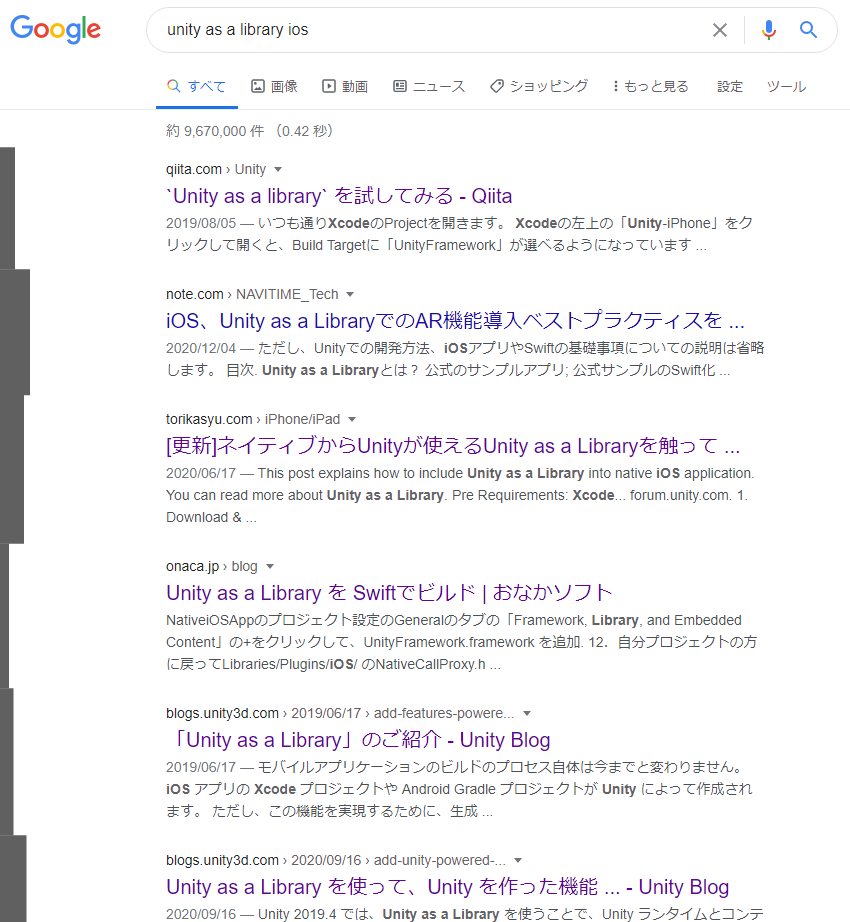
\includegraphics[width=60mm]{images/telomere.png}}
  \end{center}
  \caption{テロメアによる視覚化}
  \label{fig:ver-telomere}
\end{figure}

\subsubsection{分類動作を取り入れたウェブ検索支援システムの構築}

森らは,検索結果の内容を吟味させる方法として,一覧画面でユーザに結果の分類行動を要求している\cite{classify}.本研究の直感的という部分に該当しないが,ユーザに各情報の鮮度を吟味させる手法として効果が期待できる.

また,再検索を行う際に原因分析をユーザが行うアプローチは,本研究に鮮度以外の尺度を設ける手段として活用できる.

\subsubsection{放送型情報配信システムのための時系列性を考慮した情報フィルタリング}

馬らは,放送型ニュース配信システムにおける情報フィルタリング手法の中で,配信情報の特徴量を定義している\cite{filtersystem}.

特徴量の中には新鮮度の項目があり,類似記事の数・類似記事の密度・内容距離・時間距離の4つの基準に基づき決定されている.

いずれも該当情報と関連のある情報が全て把握できている前提があるため,Web 検索で利用することはできない.

\subsubsection{WebSCAN:Webサイトの変更発見と放送型変更通知}

WebSCAN\cite{webscan} は,Web サイトの変更を監視しその変更の価値を評価してユーザに配信する.変更の価値を評価する尺度として,新鮮度・流行度・アクセス頻度・更新頻度などを用いている.

変更通知を主題としているため,新鮮度を算出する際に,変更内容の量や質を参考にしている.本研究では更新日時のみを鮮度の尺度としてるが,更新内容まで取得できれば,よりユーザにとって有益な鮮度の表示ができる.
